\documentclass[twoside,11pt]{article}

\usepackage{aa228-jmlr2e}
\usepackage{amsmath}
\usepackage{graphicx}
\usepackage{lipsum}
\usepackage{listings}
\usepackage{url}
\usepackage{cleveref}
\usepackage{subcaption}

\usepackage{enumitem}
\usepackage{breakurl}
\usepackage{hyperref}

\setlist[itemize]{noitemsep}  % or \setlist[itemize]{itemsep=0pt, topsep=0pt}

\begin{document}

% More details can be found here: https://aa228.stanford.edu/final-project/
\title{Final Project: POMDP Navigation performance for Orienteering}

%===========================================
% Fill in your names and emails
%===========================================
\name{Stuart Johnson}
\email{stujohn@stanford.edu}

\maketitle

\section{Introduction}
At a typical orienteering event, the runner is confronted with numerous challenges: physical, strategic and navigation. The runner must not only establish a route, but also maintain and update awareness of position - without benefit of satellite positioning hardware! In this project, a basic POMDP is developed which should serve as a starting point for further development as a planning tool for events. Some aspects of an orienteering POMDP and its SARSOP solution are analyzed for a simplified, synthetic event map of a modest size.

\section{Orienteering}

Orienteering (\url{https://www.baoc.org/wiki/Welcome}) is a challenging activity and sport which combines running, route and control point finding and route planning. Control points are stations/devices placed across the orienteering course - typically part of a park. While there are several varieties of events and scoring, for the purposes of this analysis we consider a variation of common orienteering events where:

\begin{itemize}
\item The runner can visit control points (CPs) in any order.
\item The scoring is based on the time between leaving a start point and arriving at a final location.
\item The runner visits all control points.
\item A map of the course - with the CPs - is available ahead of time.
\end{itemize}

Generally, orienteering events are in moderately complex terrain with trails, roads, elevation changes, areas of difficult running and/or navigation, and control points which are a challenge to find - from a distance, anyways. A POMDP is an appropriate model - in the simplified case considered here - because our position is uncertain.

The primary goal of the POMDP planner is the generation of an optimal route and suggestions on strategy - e.g., when and where to check the map. This is a perfect scenario for offline planning. While it might be possible to provide action suggestions during a race via smartphone, it is not clear if this fits into the (rather anti-technology) rules of orienteering. A more likely scenario is a transfer of strategies found by the planner (e.g., where to check your map) to the human runner.

\section{Previous work}

Much literature (e.g. \cite{opsurvey}) applies to the Orienteering Problem (OP) and its many variants. The underlying (MDP) traveling-salesman problem is the core of the optimal route problem. Uncertainty of various types have been considered, especially in the context of robotics (e.g. \cite{figop}). However, our interest here is really in understanding, modeling and manipulating how a human interacts with the map and location uncertainty (e.g. \cite{humanop}). Thus, our POMDP components (e.g., observation model) should reflect human perception and behavior.

\section{The POMDP}

Defining the POMDP related to human localization and progress in an orienteering competition reveals numerous subtleties related to how we interact with the map. We briefly describe each component of the POMDP.

\subsection*{States}

The state is a combination of our current location (a grid world allowing diagonal movement) and whether or not we have visited our control points. An additional state is the terminal state - which has location $(-1,-1)$. The state space dimension is therefore $| \mathcal{S} | = n_x n_y 2^{n_{cp}} + 1$ where $n_{cp}$ is the number of control points.

\subsection*{Actions}
There are 9 actions:

\begin{verbatim}
const BASIC_ACTIONS_DICT =
Dict(
:MapCheck => 1,
:north => 2,
:northeast => 3, 
:east => 4,
:southeast => 5,
:south => 6,
:southwest => 7,
:west => 8,
:northwest => 9,
)
\end{verbatim}

\subsection*{Transition}

For this simple POMDP, the key to modeling human navigation/route progress on terrain is a stochastic component of the transition function. In this case, we treat our actual movement direction as a distribution about the intended bearing (action). In our case, the probability of transition is:

\begin{align*}
p_{left} = & p(\bmod(a-3,8)+2) = (1-p_a)/2 \\
p_{center} = & p(a) = p_a \\
p_{right} = & p(\bmod(a-1,8)+2) = (1-p_a)/2
\end{align*}

where this looks a little peculiar due to movement actions beginning at action 2 instead of 1. I use $p_a = 0.7$ in the examples below. In reality, $p_a$ will be a function of position on the map - in dense woods, it could be smaller. In other map regions with good visibility, $p_a$ might be closer to $1.0$.

There is other logic in the transition function to insure certain rewards are only rewarded once - and so are terminal states or sub-states.

\subsection*{Reward}

Rewards are (values used in the results section are shown):

\begin{itemize}
\item step penalty (increased by $\sqrt{2}$ for diagonal moves): -1
\item control point rewards (with POMDP logic for 1x accrual): CP1: 25, CP2: 20
\item exit reward (with POMDP logic for 1x accrual): 20
\item MapCheck penalty (this takes time): -1
\end{itemize}

\subsection*{Observation}

The observation space encodes the probability that the runner is at a position on the map, given the assessment of the runner. The dimension of the observation space is $| \mathcal{O} | = n_x n_y + 1$.The additional observation corresponds to the lack of an observation. We abuse notation in this section in that observations only care about state \textit{position}. There is no uncertainty in the state of the control points (i.e, whether or not the runner has visited them). 

\begin{itemize}
\item If we are at known landmark $s_l$, where $s_l \in \{cp_0,cp_1,...,s_{init},s_{exit}\}$, regardless of action:
\begin{equation*}
O(o|s_l,a) = \delta_{s_l}(o)
\end{equation*}
where $\delta_x(y)=0$ if $x \neq y$.
\item Else, if $a \notin $ MapCheck,
\begin{equation*}
O(o|s,a) = \delta_{o_n}(o)
\end{equation*}
where $o_n$ is the non-observation observation. This implies we propagate belief purely via the transition function.
\item Else ($a$ = MapCheck):
\begin{align*}
O(o|s,a) &\propto \mathcal{N}(o-s,\Sigma)\\
O(o_l|s_l,a) &= 0
\end{align*}
where $o_l$ is the observation corresponding to the location of $s_l$.
We only get non-zero probability of being at known landmarks $s_l$ if we are the landmark. $\Sigma$ is a diagonal covariance matrix with entries $\sigma^2$. The multivariate Gaussian is only a convenient choice for early development of the observation model (although note the final distribution may have holes in it due to landmarks). A human assessment of location is likely not to be Gaussian - nor even uni-modal.
\end{itemize}

\section{Solutions and Metrics}

The Julia POMDP packages (POMDPs, SARSOP) (\cite{egorov2017pomdps}, \cite{Kurniawati-RSS08}, \cite{Ong2009POMDPsFR}) were used to implement the solution to route planning and following with position uncertainty. This implementation was a natural modification of the RockSample.jl (\url{https://github.com/JuliaPOMDP/RockSample.jl}) POMDP example, which differs from this problem in the type and source of state uncertainty.

The solver used for this problem was SARSOP. State spaces for the maps chosen have dimension $< 1000$ and reasonably good approximations can be computed with SARSOP in minutes or hours. A SARSOP solution provides an alpha vector policy, each alpha vector tagged with an action (\cite{Kochenderfer2022}, \cite{Kurniawati-RSS08}). More algorithmic work is likely needed to scale to realistic orienteering maps. It is also possible that maps could be reduced to more compact graphs (\cite{figop}).

SARSOP policies are evaluated in simulation for a simple $10 \times 10$, 2-control point (2CP) map scenario - see  table \ref{tab:sarsopperf}. An example time step of interest is shown in figure \ref{fig:mapcheckaction}. Two metrics are defined in terms of how well the planning algorithm navigates the course. Since we are primarily interested in how navigation effects our race performance, we choose two measures of route time inflation. Assuming a constant velocity, the number of steps until simulation reaches the terminal state is a proxy for the route time. An inflation of route time over the best possible (no position uncertainty or fully-observed MDP) route time of $50\%$ is defined as a "bad" navigation outcome. A doubling of the route time over the best route time is "catastrophic". The associated metrics are the probabilities of these navigation outcomes: $p_b$ ("bad") and $p_c$ ("catastrophic"). These are estimated from 1000 simulations. Route time inflation (statistically) may be exacerbated by the POMDP solver, but it is an intrinsic feature of the POMDP - due to the stochastic dynamics and the observation function.

The best route/route time can be solved using SARSOP as follows: set the transition to deterministic (set $p_a = 1$). SARSOP discovers by itself that there is no advantage to MapChecks - propagating position belief forward with the deterministic transition function gives a perfect estimate of true position. For 2CP, the optimal route time is 18 (steps). For the solver and each simulation (see below), the position belief is initialized to the known initial position. 

\vspace{10pt}
\begin{center}
	\begin{tabular}{|c|c|c|c|c|c|c|c|c|c|c|}
	    \hline
	    \textbf{scenario/run} & $n_s$ & $\gamma$ & $t_S$ & $\delta_S$ & $n_{\alpha}$ &
	     $p_a$ & $\sigma^2$ & $t_{ref}$ & $p_b$ & $p_c$ \\
	    \hline\hline
	    2CP & 401 & 0.8 & 1200s & 0.17 & 13719 & 0.7 & 0.5 & 18 & 0.34 & 0.06\\
	    2CP1hr & 401 & 0.8 & 3600s & 0.14 & 24502 & 0.7 & 0.5 & 18 & 0.35 & 0.08 \\
	    \hline
	\end{tabular}
	\captionof{table}{SARSOP solution and navigation performance.}
	\label{tab:sarsopperf}
\end{center}


The parameters in table columns are:
\begin{itemize}[noitemsep, topsep=0pt]
\item $n_s$ : number of states
\item $\gamma$ : discount factor (for SARSOP solve). Note this is a compromise for computation time. 
\item $t_S$ : SARSOP max time parameter (SARSOP solver time)
\item $\delta_S$ : SARSOP solution precision (upper-lower bound)
\item $n_{\alpha}$ : SARSOP solution alpha vector count
\item $\sigma^2$ : POMDP observation MapCheck position estimate variance
\item $p_a$ : POMDP transition function bearing fidelity
\item $t_{ref}$ : reference path step count
\item $p_b$ : probability of a bad navigation outcome (simulation)
\item $p_c$ : probability of a catastrophic navigation outcome (simulation)
\end{itemize}

The behavior of SARSOP policies is quite interesting. As the belief slowly drifts from the true position and then spreads out near each control point (see figure \ref{fig:mapcheckaction}), the SARSOP policy finally decides to begin MapCheck actions. In other words, the control is - in the vicinity of the POMDP parameters studied - to use dead reckoning until a lack of arrival at CPs, then proceed to MapCheck. When each CP is acquired, the belief collapses again to a single grid cell, and the navigation to the next point of interest begins. Figure \ref{fig:mapcheckposition} is a 2D histogram of true runner positions when a MapCheck is made. Figure \ref{fig:routestepshist} (in the appendix) shows the long tail of difficult navigation episodes for this set of 1000 simulations. This histogram is the full picture of performance which is distilled into the $p_b$ and $p_c$ metrics.

\begin{minipage}{\textwidth}
	\begin{center}
		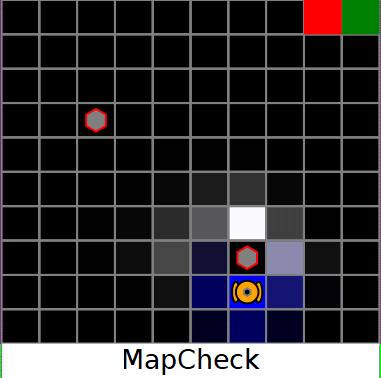
\includegraphics[width=0.5\linewidth]{../policy_2cp_1200x2_4_8.jpg}
		\captionof{figure}{Example of a MapCheck action executed by the planner. The hexagons are control points (red = not yet visited), the white/grayscale indicates current position belief, and the blue is the result of the MapCheck observation (higher opacity means higher probability). Note that the blue observation probabilities do NOT extend to the nearby control point (see the Observation section)! The round yellow object is the true runner location (a turtlebot icon, actually.) Collected from a gif rendering of a simulated course. Green and red squares are the course start and end locations.}
		\label{fig:mapcheckaction}
	\end{center}
\end{minipage}

\begin{minipage}{\textwidth}
	\begin{center}
		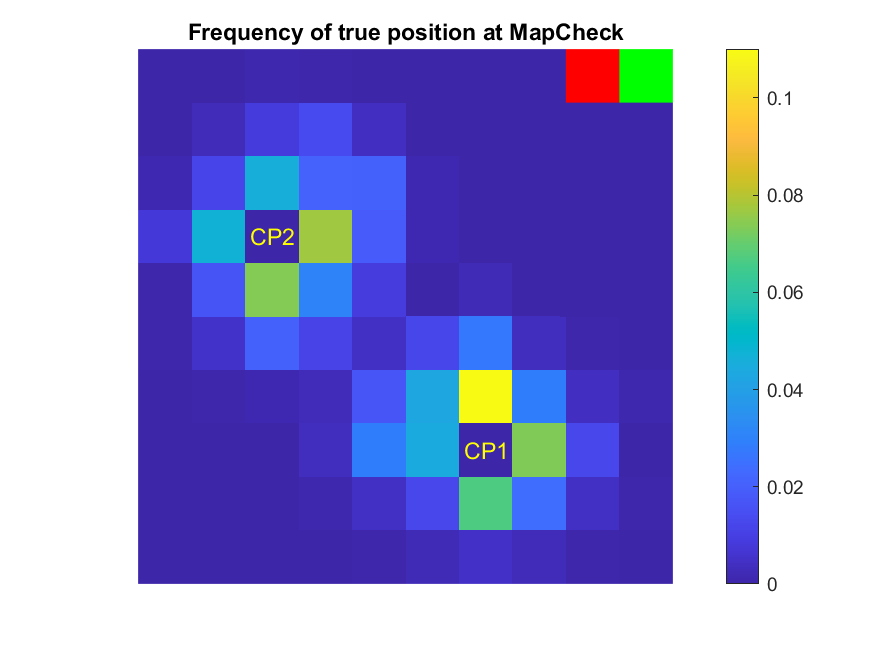
\includegraphics[width=0.8\linewidth]{../MapCheckPosition.jpg}
		\captionof{figure}{True position of runner when executing MapCheck. Collected from 1000 simulated routes.}
		\label{fig:mapcheckposition}
	\end{center}
\end{minipage}


\section{Conclusions and future work}

Given the metrics computed in the previous section, a bad outcome at the (synthetic) race is quite likely. More modeling of transition dynamics and navigation uncertainty are in order. When using the planner on a real course map, we expect more subtlety in action choice than "Use dead reckoning!". Given the run time of SARSOP, a more scalable approach will be needed for realistic course maps.

This POMDP is just a first step in a more thorough implementation of an orienteering planner. However, even a simple POMDP can be a challenge to understand, implement and solve; development should proceed in small steps. A real orienteering race adds many complexities, including:

\begin{itemize}[noitemsep, topsep=0pt]
\item Route confusion (the stochastic transition) is (strongly) a function of position on the map
\item Position uncertainty (the observation) is strongly a function of position on the map.
\item Terrain uncertainty exists in typical orienteering courses. For example, the penalty for traversing some terrain may be quite high. This may cause the planner to be more cautious near difficult terrain - but, on the other hand, it may be useful to explore some terrain if significant time savings exist.
\item Course map ingestion and processing (into a POMDP, for example) will be a significant effort for a working planner. 
\end{itemize}


% References
\bibliography{references}

\section{Appendix}

\begin{minipage}{\textwidth}
	\begin{center}
		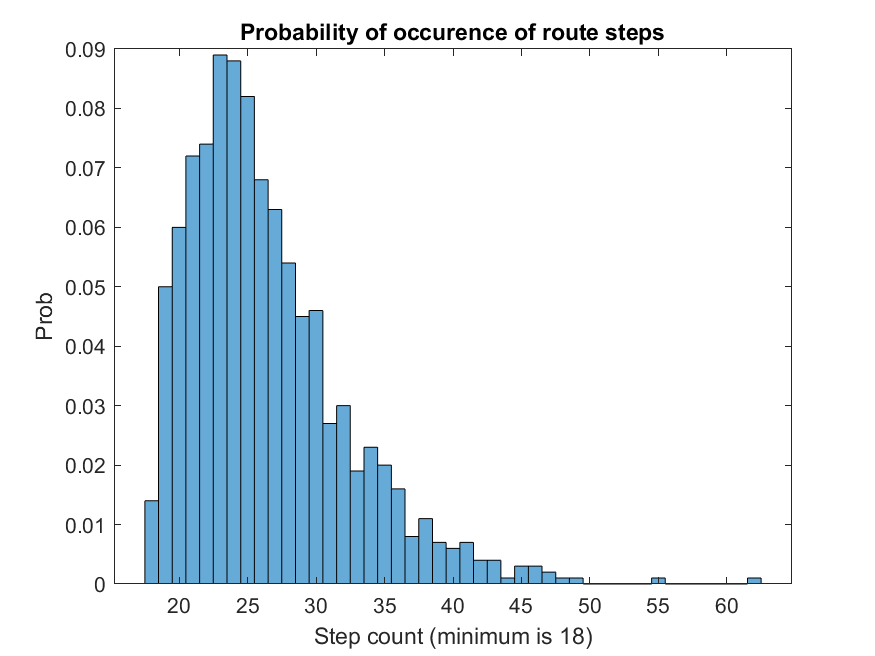
\includegraphics[width=0.8\linewidth]{../RouteStepsHist.png}
		\captionof{figure}{Histogram of route steps - a proxy for time on course. Collected from 1000 simulated routes. The $p_c$ and $p_b$ metrics are measures of this distribution.}
		\label{fig:routestepshist}
	\end{center}
\end{minipage}

\end{document}

